\setlength\parindent{8pt}
In computer vision area with Convolutional Neural Network(CNN), it is quite common that replacing 5x5 convolution kernels by two of 3x3 kernels to reduce the computational cost\cite{Inception}. However for RNN-like cells, there are few or none of such things due to the complexity of the cell.

In this proposal, we will introduce a Recurrent Neural Network(RNN) structure that is efficient in the aspect of number of parameters. RNN(and its variants) is a basic neural network cell that works very well on sequential inputs so widely adopted for Natural Language Processing(NLP), video processing etc. It is composed of hidden layer and output layer. Hidden layer is a layer that feed RNN status to next RNN and fed by previous RNN, and output layer is a layer that gives actual output of network.

Improving the performance of the RNN cell, one common choice is increasing the number of the hidden parameters. However, this approach is not possible for many users. Making hidden layer requires huge amount of memory and computational power but most RNN users are not affordable for it. Also, making RNN hidden layer bigger is risky because it tends to overfit when we increase the size of hidden layer. So our object is to find a novel approach to reduce those cost while keeping its performance as much as possible.

There are not that much works that deals with this problem directly. However, inspired by the technique explained above(replacing 5x5 kernel by two of 3x3), we came up with a brand new approach that factorizing a huge RNN cell into small cells. One approach for this is explained on Figure \ref{fig:RNNcell1}. The figure shows the factorized RNN cells with smaller hidden layer size. Initially, the input only goes to cell 1 and updates the hidden state of the cell. For following input, we use the hidden state of the cell1 to determine which cell to use to process the input. We then repeat this until the end of the input sequence.
\begin{figure}
  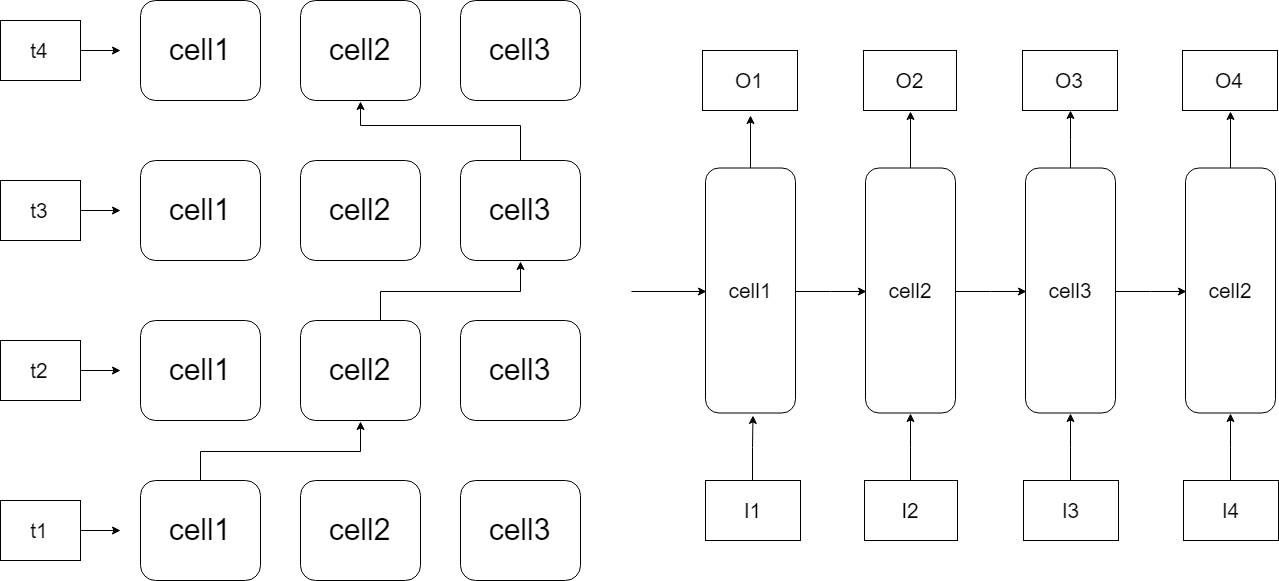
\includegraphics[width=\linewidth]{pictures/RNNfig1.png}
  \caption{One kind of example figure for factorized RNN cells.}
  \label{fig:RNNcell1}
\end{figure}
$$h_t = \sigma(W_hx_t+U_hh_{t-1}+b_h)\label{Elman}$$
$$y_t = \sigma_y(W_yh_t+b_y)$$
\cite{Elman90}

From Elman network which is fully recurrent network, can represent equation \ref{Elman}. Suppose size of hidden layer and size of input size as $n$ and $k$ each. To get hidden state of Elman network we need $n^2+nk+n$ parameters. Let us factorize the cell into 3 cells. Than hidden size become $\frac{n}{3}$ in this network we need $3(\frac{n}{3}^2+\frac{n}{3}k+\frac{n}{3}) = \frac{n^2}{3}+nk+n$. This consider total parameter in RNN cells. In real computation we do not update whole parameter in RNN cells. Thus, in real computation, we can expect less cost.


